\documentclass{article}
\usepackage{tikz}
\usetikzlibrary{matrix,chains,positioning,decorations.pathreplacing,arrows}

\begin{document}

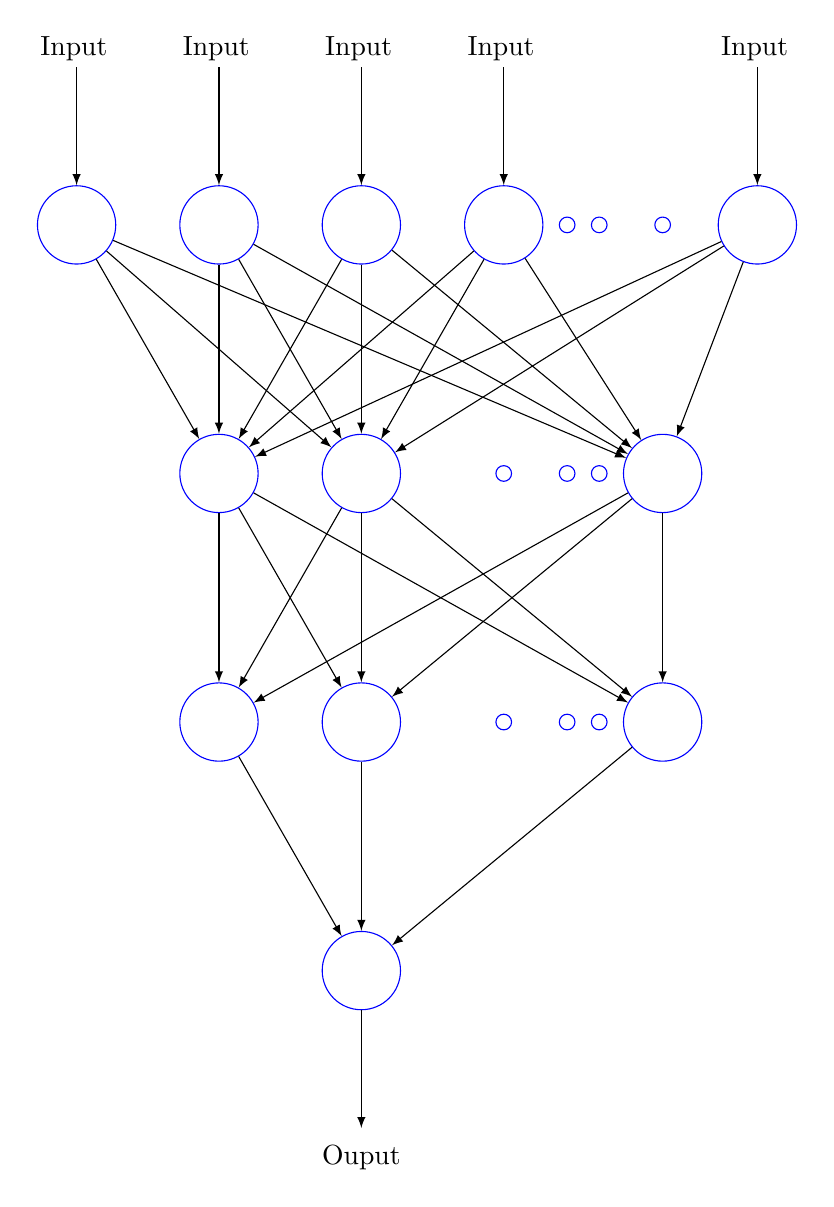
\begin{tikzpicture}[
plain/.style={
  draw=none,
  fill=none,
  },
dot/.style={draw,shape=circle,minimum size=3pt,inner sep=0,fill=black
  },  
net/.style={
  matrix of nodes,
  ampersand replacement=\&,
  nodes={
    draw,
    circle,
    color=blue,
    inner sep=10pt
    },
  nodes in empty cells,
  column sep = 0.8cm,
  row sep=-10pt
  },  
>=latex]
\matrix [net] (mat)
{
	\& \& \& \&[-4ex] |[inner sep=2pt]|\&[-4ex] |[inner sep=2pt]|\&[-4ex] |[inner sep=2pt]|\&[-4ex] \\[25mm]
	|[plain]| \& \& \&[-4ex] |[inner sep=2pt]|\&[-4ex] |[inner sep=2pt]|\&[-4ex] |[inner sep=2pt]|\& \\ [25mm]
	|[plain]| \& \& \&[-4ex] |[inner sep=2pt]|\&[-4ex] |[inner sep=2pt]|\&[-4ex] |[inner sep=2pt]|\& \\ [25mm]
	|[plain]|\& 
	|[plain]| \&  \\
};

\foreach \inn in {1,2,3,4,8}
	\draw[<-] (mat-1-\inn) -- node[above] [shift={(-1pt,20pt)}]{Input} +(0,+2cm);


\foreach \ai in {1,2,3,4,8}
{\foreach \aii in {2,3,7}
  \draw[->] (mat-1-\ai) -- (mat-2-\aii);  
}
\foreach \ai in {2,3,7}
{\foreach \aii in {2,3,7}
  \draw[->] (mat-2-\ai) -- (mat-3-\aii);  
}
\foreach \ai in {2,3,7}
{\foreach \aii in {3}
  \draw[->] (mat-3-\ai) -- (mat-4-\aii);  
}
\draw[->] (mat-4-3) -- node[above] [shift={(0pt,-40pt)}]{Ouput}+(0,-2cm);




\end{tikzpicture}


\end{document}
